\section{Proofs}
\subsection{Proof of Proposition~\ref{prop:gaussian_var_inflation}}
\label{app:proof_of_var_inflation_multi_dim}
\begin{proof}[Proof: Inflation of Gaussian policy variance (multidimensional perspective)]

Under the local first-order approximation,
\[
\hat Q(s,a)=\hat Q(s,\mu)+g^\top(a-\mu)+o(\|a-\mu\|_2),
\qquad g\neq 0.
\]
Since
\[
a_k=\mu+\sigma\odot \epsilon_k,
\qquad
\epsilon_k\overset{i.i.d.}{\sim}\mathcal N(0,I),
\]
the first-order term becomes
\[
g^\top(a_k-\mu)
=
g^\top(\sigma\odot \epsilon_k)
=
(\sigma\odot g)^\top \epsilon_k.
\]
Define
\[
w\coloneq \sigma\odot g.
\]
Then, up to the local first-order approximation, the winner index is
\[
k^*\in \arg\max_{1\le k\le K} w^\top \epsilon_k.
\]
Let
\[
u\coloneq \frac{w}{\|w\|_2}.
\]
For each sample $\epsilon_k$, decompose it as
\[
\epsilon_k=z_k u+\xi_k,
\]
where
\[
z_k\coloneq u^\top \epsilon_k \sim \mathcal N(0,1),
\qquad
\xi_k \perp u,
\qquad
z_k \text{ is independent of } \xi_k.
\]
Since
\[
w^\top \epsilon_k = \|w\|_2 z_k,
\]
the winner index is equivalently
\[
k^*=\arg\max_{1\le k\le K} z_k.
\]
Hence the selected noise can be written as
\[
\epsilon^* \coloneq \epsilon_{k^*}= z_{(K)}u+\xi^*,
\qquad
z_{(K)}\coloneq \max_{1\le k\le K} z_k,
\]
where $\xi^*$ has the same distribution as the orthogonal component of a standard Gaussian sample and remains independent of $z_{(K)}$.

Now consider the winner-MLE loss
\[
\mathcal L(\mu,\sigma;s)=-\log \pi_{\mu,\sigma}(a^*|s),
\qquad
a^*=\mu+\sigma\odot \epsilon^*,
\]
with $a^*$ treated as a fixed target. For a diagonal Gaussian policy,
\[
\mathcal L
=
\sum_i \left(
\log \sigma_i + \frac{(a_i^*-\mu_i)^2}{2\sigma_i^2}
\right)+C,
\]
where $C$ is constant with respect to $(\mu,\sigma)$. Therefore,
\[
\frac{\partial \mathcal L}{\partial \log \sigma_i}
=
1-\frac{(a_i^*-\mu_i)^2}{\sigma_i^2}
=
1-(\epsilon_i^*)^2.
\]
Taking expectation,
\[
\mathbb E\!\left[\frac{\partial \mathcal L}{\partial \log \sigma_i}\right]
=
1-\mathbb E[(\epsilon_i^*)^2].
\]

Using $\epsilon_i^*=u_i z_{(K)}+\xi_i^*$, we obtain
\[
\mathbb E[(\epsilon_i^*)^2]
=
u_i^2 \mathbb E[z_{(K)}^2]
+
2u_i \mathbb E[z_{(K)}\xi_i^*]
+
\mathbb E[(\xi_i^*)^2].
\]
The cross term vanishes by independence and zero mean of the orthogonal component:
\[
\mathbb E[z_{(K)}\xi_i^*]=0.
\]
Moreover, since a standard Gaussian has unit covariance and $u$ is unit norm,
\[
\mathbb E[(\xi_i^*)^2]=1-u_i^2.
\]
Therefore,
\[
\mathbb E[(\epsilon_i^*)^2]
=
u_i^2 \alpha_K + (1-u_i^2),
\qquad
\alpha_K\coloneq \mathbb E[z_{(K)}^2].
\]
Substituting back,
\[
\mathbb E\!\left[\frac{\partial \mathcal L}{\partial \log \sigma_i}\right]
=
1-\big(u_i^2\alpha_K + 1-u_i^2\big)
=
-(\alpha_K-1)u_i^2.
\]
For $K\ge 3$, we have $\alpha_K>1$, so
\[
\mathbb E\!\left[\frac{\partial \mathcal L}{\partial \log \sigma_i}\right]\le 0,
\]
with strict inequality whenever $u_i\neq 0$, equivalently whenever $(\sigma_i g_i)\neq 0$.
This proves the claim.
\end{proof}

\subsection{Proof of Proposition~\ref{prop:inf_var_lower_Q} and Corollary~\ref{cor:persistent_variance_return_gap}}
\label{app:proof_inf_var_lower_Q_ret}
\begin{proof}[Proof: Inflated variance lowers $Q$ and return]
    For an arbitrary fixed state $s$, assume that $Q(s,a)$ is locally $m$-strongly concave around the optimal action $a^*(s)$, and that there exists a constant $m>0$ such that
\begin{equation}
    Q(s,a)\le Q\bigl(s,a^*(s)\bigr)-\frac{m}{2}\|a-a^*(s)\|^2,
\end{equation}
for all $a$ in a neighborhood of $a^*(s)$.

Consider a Gaussian policy $a \sim \pi(\cdot|s)=\mathcal{N}\bigl(\mu(s),\Sigma(s)\bigr)$, where $\Sigma(s)=\mathrm{diag}(\sigma^2(s))$. Assume the policy is locally converged in the sense that $\mu(s)=a^*(s)$. Then
\begin{equation}
    \mathbb{E}_{a\sim\pi(\cdot|s)}[Q(s,a)]
    \le
    Q\bigl(s,a^*(s)\bigr)
    -\frac{m}{2}\,
    \mathbb{E}_{a\sim\pi(\cdot|s)}\|a-a^*(s)\|^2.
\end{equation}
For the Gaussian policy above,
\begin{equation}
    \mathbb{E}_{a\sim\pi(\cdot|s)}\|a-a^*(s)\|^2
    = \mathrm{tr}\bigl(\Sigma(s)\bigr)
    = \sum_i \sigma_i^2(s),
\end{equation}
and therefore
\begin{equation}
    \mathbb{E}_{a\sim\pi(\cdot|s)}[Q(s,a)]
    \le
    Q\bigl(s,a^*(s)\bigr)
    -\frac{m}{2}\sum_i \sigma_i^2(s).
\end{equation}
Under the assumptions of Proposition~\ref{prop:inf_var_lower_Q}, suppose additionally that for every state $s$ visited by $\pi$, the action $a^*(s)$ maximizes $Q^{\pi^*}(s,a)$, i.e.,
\begin{equation}
    a^*(s)\in \arg\max_a Q^{\pi^*}(s,a),
\end{equation}
and the local quadratic upper bound holds on the support of $\pi(\cdot\mid s)$. Then
\begin{equation}
    J(\pi^*)-J(\pi)
    \ge
    \frac{m}{2(1-\gamma)}
    \mathbb{E}_{s\sim d^\pi}\!\left[\operatorname{tr}(\Sigma(s))\right].
\end{equation}
For diagonal covariance $\Sigma(s)=\operatorname{diag}(\sigma_1^2(s),\dots,\sigma_d^2(s))$, this becomes
\begin{equation}
    J(\pi^*)-J(\pi)
    \ge
    \frac{m}{2(1-\gamma)}
    \mathbb{E}_{s\sim d^\pi}\!\left[\sum_{i=1}^d \sigma_i^2(s)\right].
\end{equation}
\end{proof}

\clearpage
\section{Additional Experimental Results}
\label{app:additional-experiments}

\begin{table}[p]
\centering
\scriptsize
\caption{Scores for DMC Hard (1M) tasks, reported as mean $\pm$ standard deviation. Each score is computed by first taking the maximum return within each seed, and then computing the mean and standard deviation across seeds. We \textbf{bold} the best result for each task.}
\label{tab:dmc_scores_with_igp}
\setlength{\tabcolsep}{3pt}
\resizebox{\linewidth}{!}{%
\begin{tabular}{lrrrrrr}
\toprule
Task & TD-MPC2 & BRC & BRC-ST & EZ-M-ST & EZ-M & EZ-IGP(ours) \\
\midrule
\texttt{dog-stand}
& $817.367{\pm}23.354$
& $945.557{\pm}35.713$
& $913.862{\pm}57.743$
& $947.730{\pm}5.045$
& $945.741{\pm}7.064$
& $\mathbf{974.790{\pm}8.358}$ \\
\texttt{dog-walk}
& $719.833{\pm}68.214$
& $809.929{\pm}147.561$
& $764.241{\pm}97.900$
& $778.395{\pm}110.429$
& $915.123{\pm}6.744$
& $\mathbf{958.983{\pm}5.187}$ \\
\texttt{dog-run}
& $228.800{\pm}22.439$
& $281.717{\pm}49.678$
& $299.228{\pm}73.987$
& $241.965{\pm}70.275$
& $405.874{\pm}50.808$
& $\mathbf{613.257{\pm}6.546}$ \\
\texttt{dog-trot}
& $500.033{\pm}16.631$
& $516.288{\pm}130.027$
& $588.662{\pm}95.487$
& $466.416{\pm}122.449$
& $815.958{\pm}76.640$
& $\mathbf{942.814{\pm}3.341}$ \\
\texttt{humanoid-stand}
& $663.733{\pm}32.515$
& $737.042{\pm}201.735$
& $751.334{\pm}166.116$
& $589.152{\pm}97.187$
& $772.273{\pm}8.943$
& $\mathbf{903.719{\pm}7.734}$ \\
\texttt{humanoid-walk}
& $628.233{\pm}16.280$
& $314.038{\pm}271.480$
& $569.773{\pm}92.383$
& $531.614{\pm}5.920$
& $779.404{\pm}39.126$
& $\mathbf{911.542{\pm}7.005}$ \\
\texttt{humanoid-run}
& $190.200{\pm}14.062$
& $62.398{\pm}73.964$
& $161.155{\pm}42.949$
& $153.026{\pm}33.236$
& $259.030{\pm}25.534$
& $\mathbf{369.468{\pm}5.633}$ \\
\bottomrule
\end{tabular}
}
\end{table}

\begin{table}[p]
\centering
\scriptsize
\caption{Scores for HumanoidBench-Hard (1M) tasks, reported as mean $\pm$ standard deviation across three seeds after taking the maximum return within each seed. We \textbf{bold} results above the success score, or the SoTA when all methods are below it.}
\label{tab:humanoidbench_hard}
\resizebox{\linewidth}{!}{%
\begin{tabular}{lrrrrrrr}
\toprule
Task & Random & Success & TD-MPC2 & BRC & BRC-ST & EZ-M & EZ-IGP(ours) \\
\midrule
\texttt{h1hand-stand}
& 11.973 & 800.0
& $209.256{\pm}52.474$ & $\mathbf{890.627{\pm}64.554}$ & $344.159{\pm}309.290$ & $\mathbf{914.460{\pm}2.127}$ & $\mathbf{899.706{\pm}11.895}$ \\
\texttt{h1hand-walk}
& 2.505 & 700.0
& $235.559{\pm}93.954$ & $622.684{\pm}139.376$ & $\mathbf{858.652{\pm}106.977}$ & $\mathbf{923.384{\pm}3.694}$ & $\mathbf{\textcolor{blue}{923.752{\pm}3.092}}$ \\
\texttt{h1hand-run}
& 1.927 & 700.0
& $35.943{\pm}3.973$ & $189.786{\pm}25.663$ & $51.847{\pm}13.318$ & $\mathbf{822.343{\pm}43.723}$ & $\mathbf{889.872{\pm}7.244}$ \\
\texttt{h1hand-stair}
& 3.161 & 700.0
& $51.033{\pm}3.398$ & $191.848{\pm}45.344$ & $65.302{\pm}11.846$ & $\mathbf{441.692{\pm}19.294}$ & $381.660{\pm}25.700$ \\
\texttt{h1hand-crawl}
& 278.868 & 800.0
& $\mathbf{898.560{\pm}35.968}$ & $740.718{\pm}59.136$ & $\mathbf{854.395{\pm}19.127}$ & $665.573{\pm}70.116$ & $647.794{\pm}59.109$ \\
\texttt{h1hand-slide}
& 3.142 & 700.0
& $97.656{\pm}16.324$ & $332.524{\pm}58.340$ & $151.583{\pm}39.211$ & $666.507{\pm}65.815$ & $\mathbf{870.521{\pm}46.518}$ \\
\texttt{h1hand-pole}
& 19.721 & 700.0
& $150.233{\pm}21.203$ & $551.138{\pm}104.690$ & $439.295{\pm}28.894$ & $\mathbf{887.945{\pm}25.582}$ & $\mathbf{879.091{\pm}9.683}$ \\
\texttt{h1hand-hurdle}
& 2.371 & 700.0
& $42.457{\pm}6.239$ & $110.333{\pm}11.177$ & $55.887{\pm}9.599$ & $\mathbf{471.050{\pm}38.269}$ & $465.969{\pm}140.063$ \\
\texttt{h1hand-maze}
& 106.233 & 1200.0
& $142.249{\pm}11.927$ & $362.677{\pm}4.216$ & $348.915{\pm}5.388$ & $451.575{\pm}12.825$ & $\mathbf{479.622{\pm}72.949}$ \\
\texttt{h1hand-sit\_simple}
& 10.768 & 750.0
& $675.884{\pm}196.728$ & $\mathbf{935.483{\pm}3.844}$ & $\mathbf{901.682{\pm}25.333}$ & $\mathbf{872.353{\pm}12.648}$ & $\mathbf{814.452{\pm}51.049}$ \\
\texttt{h1hand-sit\_hard}
& 2.477 & 750.0
& $148.216{\pm}36.804$ & $\mathbf{885.141{\pm}33.683}$ & $710.754{\pm}258.261$ & $358.350{\pm}10.554$ & $\textcolor{blue}{426.718{\pm}30.742}$ \\
\texttt{h1hand-balance\_simple}
& 10.170 & 800.0
& $27.412{\pm}3.310$ & $101.305{\pm}8.963$ & $106.005{\pm}6.567$ & $103.400{\pm}12.201$ & $\mathbf{310.167{\pm}17.553}$ \\
\texttt{h1hand-balance\_hard}
& 10.032 & 800.0
& $33.042{\pm}6.165$ & $72.918{\pm}2.266$ & $\mathbf{77.788{\pm}5.622}$ & $74.962{\pm}4.581$ & $70.913{\pm}8.696$ \\
\texttt{h1hand-reach}
& -50.024 & 12000.0
& $3610.454{\pm}617.640$ & $4317.026{\pm}1527.201$ & $4931.460{\pm}597.736$ & $\mathbf{5820.811{\pm}501.354}$ & $5114.852{\pm}40.931$ \\
\bottomrule
\end{tabular}
}
\end{table}

\begin{table}[t]
\centering
\small
\caption{\textcolor{blue}{Refinement-matched comparison on DMC humanoid tasks (mean $\pm$ sample standard deviation over three seeds).}}
\label{tab:matched_gaussian_refine}
\begin{tabular}{lcc}
\toprule
Task & Gaussian + Refine & EZ-IGP \\
\midrule
\texttt{humanoid-stand} & $763.8\pm18.7$ & $\mathbf{903.7\pm7.7}$ \\
\texttt{humanoid-walk} & $761.6\pm35.5$ & $\mathbf{911.5\pm7.0}$ \\
\texttt{humanoid-run} & $230.5\pm37.5$ & $\mathbf{369.5\pm5.6}$ \\
\bottomrule
\end{tabular}
\end{table}

\noindent\textbf{Matched-Gaussian details.}
The Gaussian control uses the same backbone, $K=8$ candidates, $N=16$
simulations per round, two refinement rounds, winner-action target, and
unchanged SEM/categorical path. Its \texttt{dist/policy\_sigma} rises from
$1.76\pm0.16$ to an early peak of $3.02\pm0.16$ and remains at
$2.11\pm0.04$ over the final 10\% of training. A separate two-seed control
that distills a search-score-weighted mixture of all candidates retains
elevated final variance ($2.67\pm0.04$) and underperforms winner-target
Gaussian distillation on the same tasks.

\begin{table}[t]
\centering
\caption{\textbf{Preliminary HB-Hard sensitivity study.} Benchmark normalized scores (mean $\pm$ sample standard deviation over three seeds), evaluated near 300k training updates across 14 tasks. Candidates/simulations are fixed at 8/16 per round; total search computation grows with $R$.}
\label{tab:hb_hard_vr_sweep}
\begin{tabular}{ccc}
\toprule
Bins $V$ & Rounds $R$ & Normalized score \\
\midrule
11 & 2 & $0.622 \pm 0.017$ \\
21 & 2 & $0.617 \pm 0.025$ \\
31 & 2 & $0.643 \pm 0.013$ \\
41 & 2 & $0.590 \pm 0.013$ \\
\midrule
31 & 1 & $0.603 \pm 0.027$ \\
31 & 4 & $0.649 \pm 0.047$ \\
\bottomrule
\end{tabular}
\end{table}

\begin{table}[t]
\centering
\small
\caption{\textcolor{blue}{DMC humanoid performance under strict search budgets (mean $\pm$ sample standard deviation).}}
\label{tab:simulation_budget}
\resizebox{\linewidth}{!}{%
\begin{tabular}{ccccc}
\toprule
Candidates / simulations & Stand & Walk & Run & Average \\
\midrule
$2/4$ & $375.193\pm10.490$ & $406.443\pm37.224$ & $108.607\pm0.046$ & $296.748\pm15.889$ \\
$4/8$ & $772.111\pm15.872$ & $790.306\pm47.157$ & $221.021\pm31.538$ & $594.479\pm31.523$ \\
$8/16$ & $903.719\pm7.734$ & $911.542\pm7.005$ & $369.468\pm5.633$ & $728.243\pm1.635$ \\
\bottomrule
\end{tabular}
}
\end{table}

\begin{figure}[t]
    \centering
    \begin{minipage}[t]{0.49\textwidth}
        \centering
        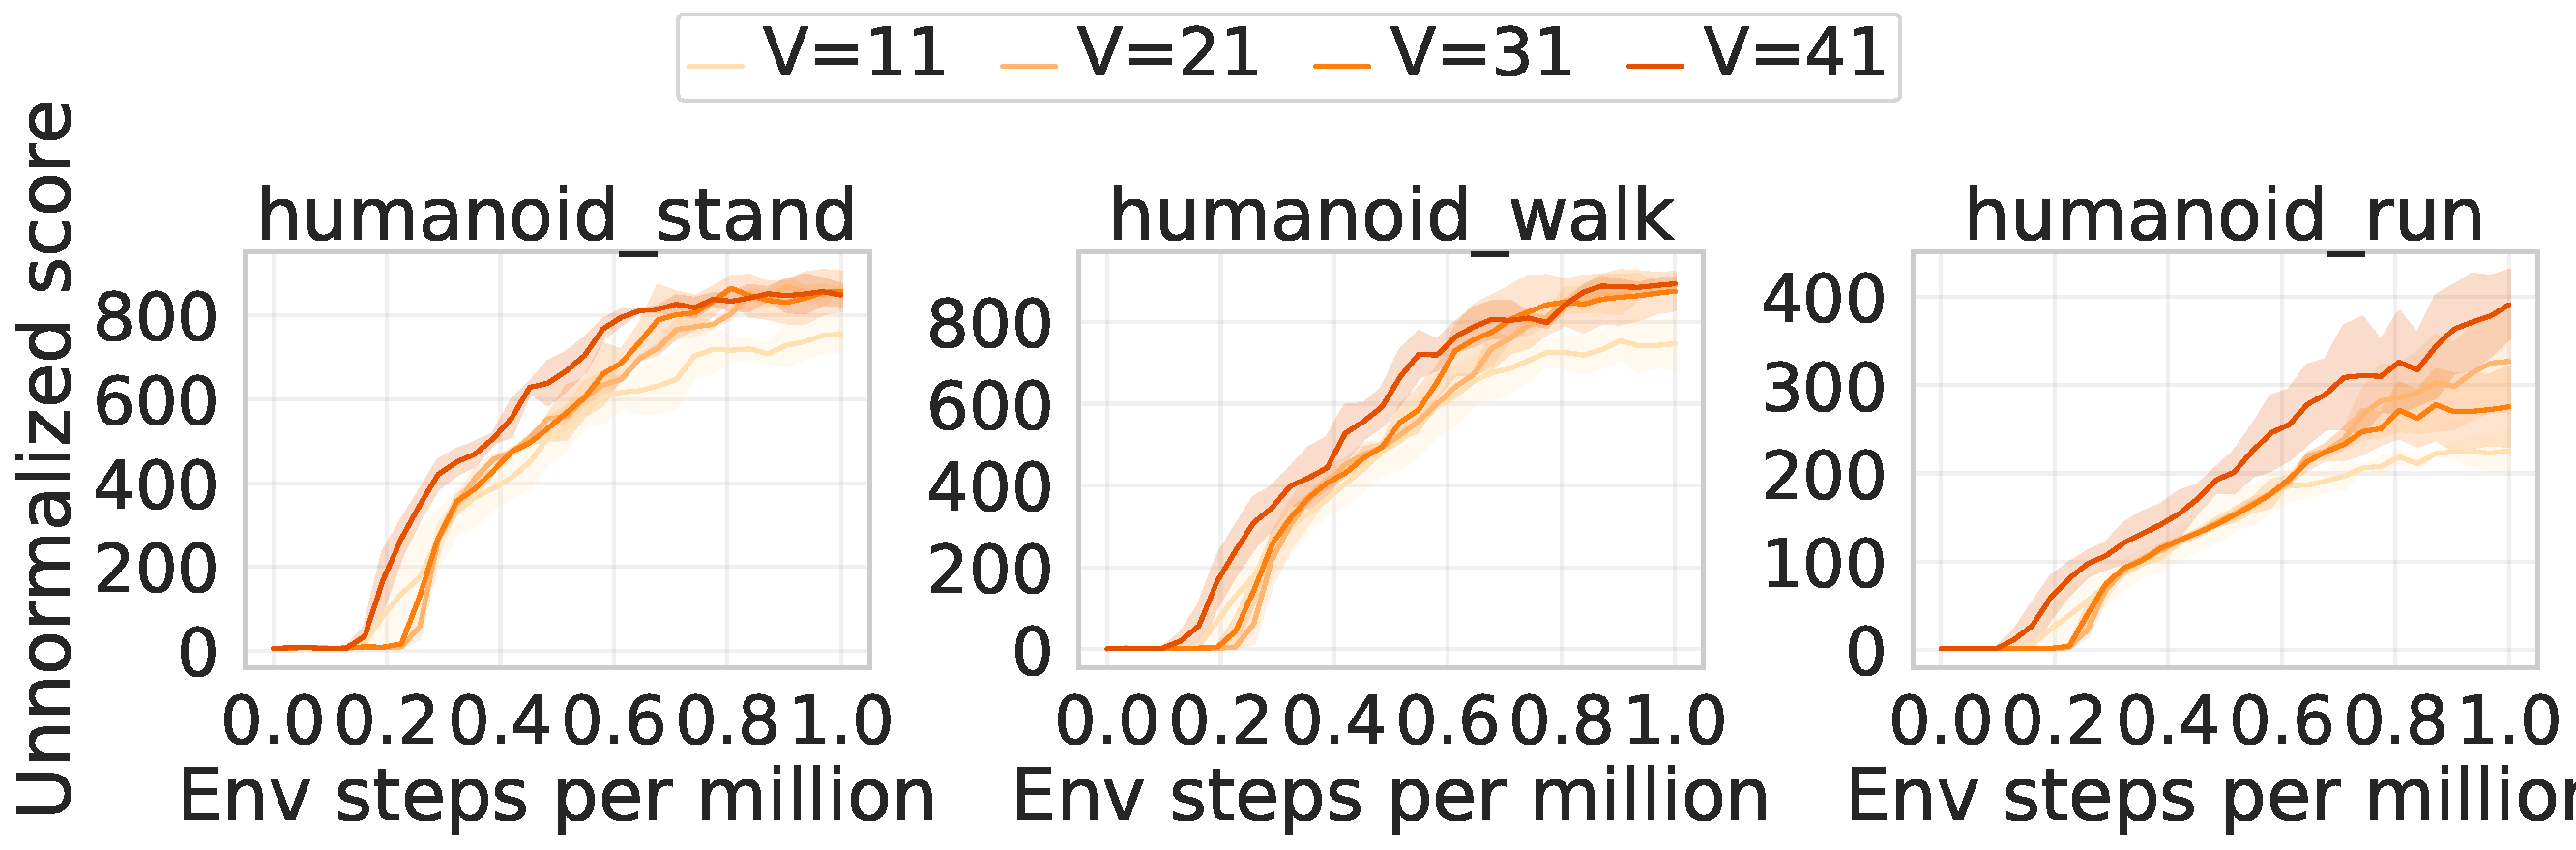
\includegraphics[width=\textwidth]{figs/V_ablation.pdf}
        \vspace{0.1cm}
        \centerline{(a) Effect of discretization granularity}
    \end{minipage}
    \hfill
    \begin{minipage}[t]{0.49\textwidth}
        \centering
        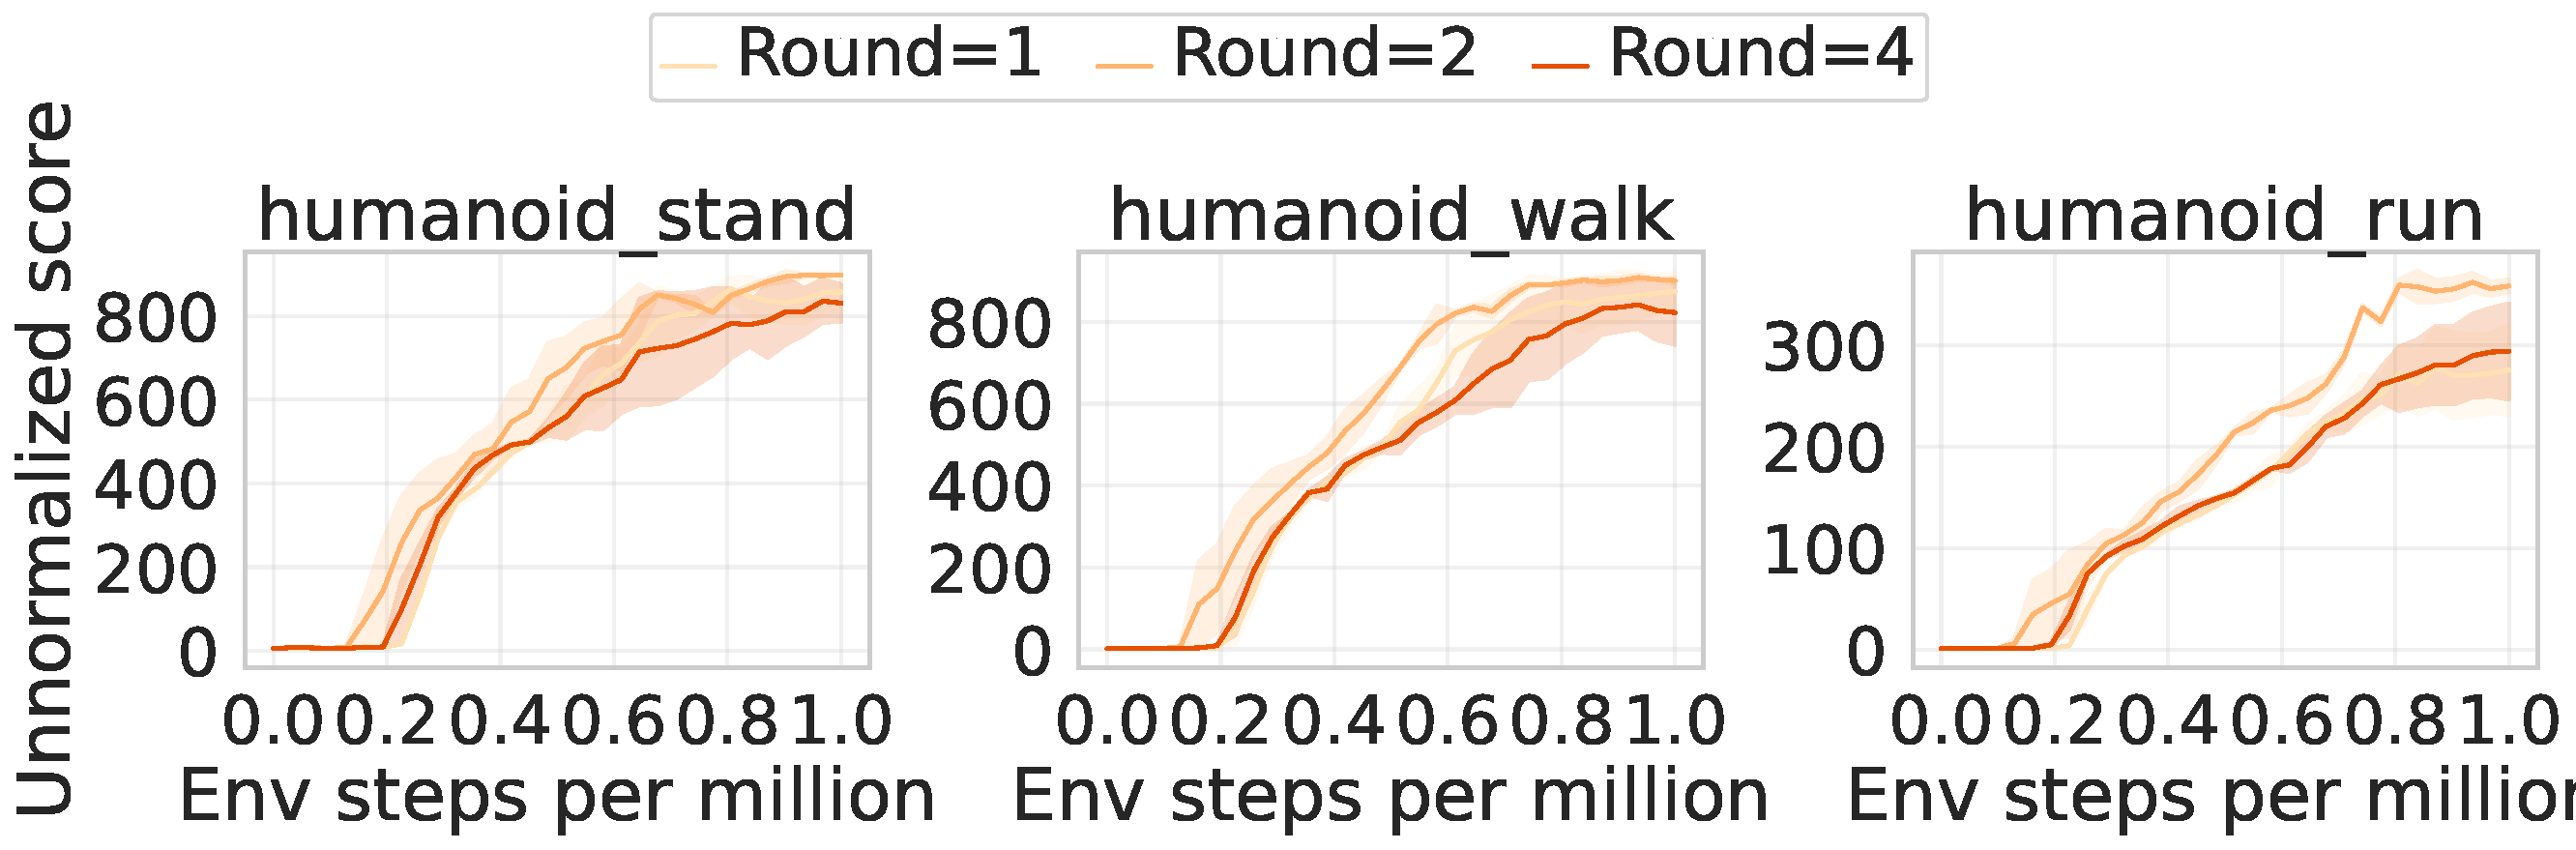
\includegraphics[width=\textwidth]{figs/Round_ablation.pdf}
        \vspace{0.1cm}
        \centerline{(b) Effect of refinement rounds}
    \end{minipage}
    \caption{\textbf{Ablation studies on three DMC humanoid tasks.} \textbf{(a)} Finer discretization improves returns on these tasks, with diminishing returns beyond $V=31$. \textbf{(b)} One or two search rounds perform well, while four rounds reduce returns on several tasks. These task-specific trends need not generalize to other benchmarks; see Table~\ref{tab:hb_hard_vr_sweep}.}
    \label{fig:ablations}
\end{figure}

\noindent\textbf{Ablation interpretation.}
On the DMC humanoid tasks, coarse discretization ($V=11$) slows learning and
lowers final returns, while $V=31$ and $V=41$ perform similarly in most cases.
One round disables proposal refinement; two rounds add one refine-and-resample
step. On the 14-task HB-Hard sweep, two rounds improve the mean over one round,
whereas four rounds add little with greater variability and twice the search
expansions. The bin count controls support resolution, while the refinement
count controls repeated proposal updates. The budget sweep shows monotonic
degradation from $8/16$ to $2/4$, consistent with reduced candidate coverage
and weaker ranking.

\clearpage
\section{Training Curves}
\label{sec:app_curves}

This section presents the full training dynamics of EZ-IGP and the baselines on the two benchmark suites used in our evaluation: the high-dimensional subset of DMControl (DMC-Hard) and HumanoidBench-Hard. While the per-task scores reported in Tables~\ref{tab:dmc_scores_with_igp} and \ref{tab:humanoidbench_hard} summarize \textit{peak} performance, they do not directly reflect how each method behaves during the course of training. The curves below complement those tables by exposing two additional dimensions of method quality: \textit{learning speed}, i.e., how quickly returns rise as a function of environment interactions, and \textit{learning stability}, i.e., how consistently performance is maintained across seeds and across the training budget.

In all figures, the $y$-axis denotes the unnormalized episodic return and the $x$-axis denotes environment steps in millions. Each curve is aggregated over 5 random seeds; solid lines correspond to the seed mean and shaded regions to 95\% bootstrap confidence intervals. We report \textit{unnormalized} returns here so that readers can directly compare to the raw scores used by prior work and to the per-task random/success thresholds listed in Table~\ref{tab:humanoidbench_hard}.

Fig.~\ref{fig:dmc-unnorm-curves} reports the curves on the 7-task DMC-Hard suite, comprising 4 dog tasks (\textit{dog-stand}, \textit{dog-walk}, \textit{dog-run}, \textit{dog-trot}) and 3 humanoid tasks (\textit{humanoid-stand}, \textit{humanoid-walk}, \textit{humanoid-run}). These two embodiment families differ markedly in morphology and physical modeling, so their joint inclusion lets us assess whether the gains from EZ-IGP transfer across embodiments rather than being tied to a specific robot. Reading the curves alongside Table~\ref{tab:dmc_scores_with_igp} also clarifies an effect that peak-score tables can hide: on the more dynamic tasks such as \textit{dog-run} and \textit{dog-trot}, EZ-IGP's advantage opens up early in training and is preserved throughout, indicating better sample efficiency rather than only a higher asymptote.

\begin{figure}[ht]
    \centering
    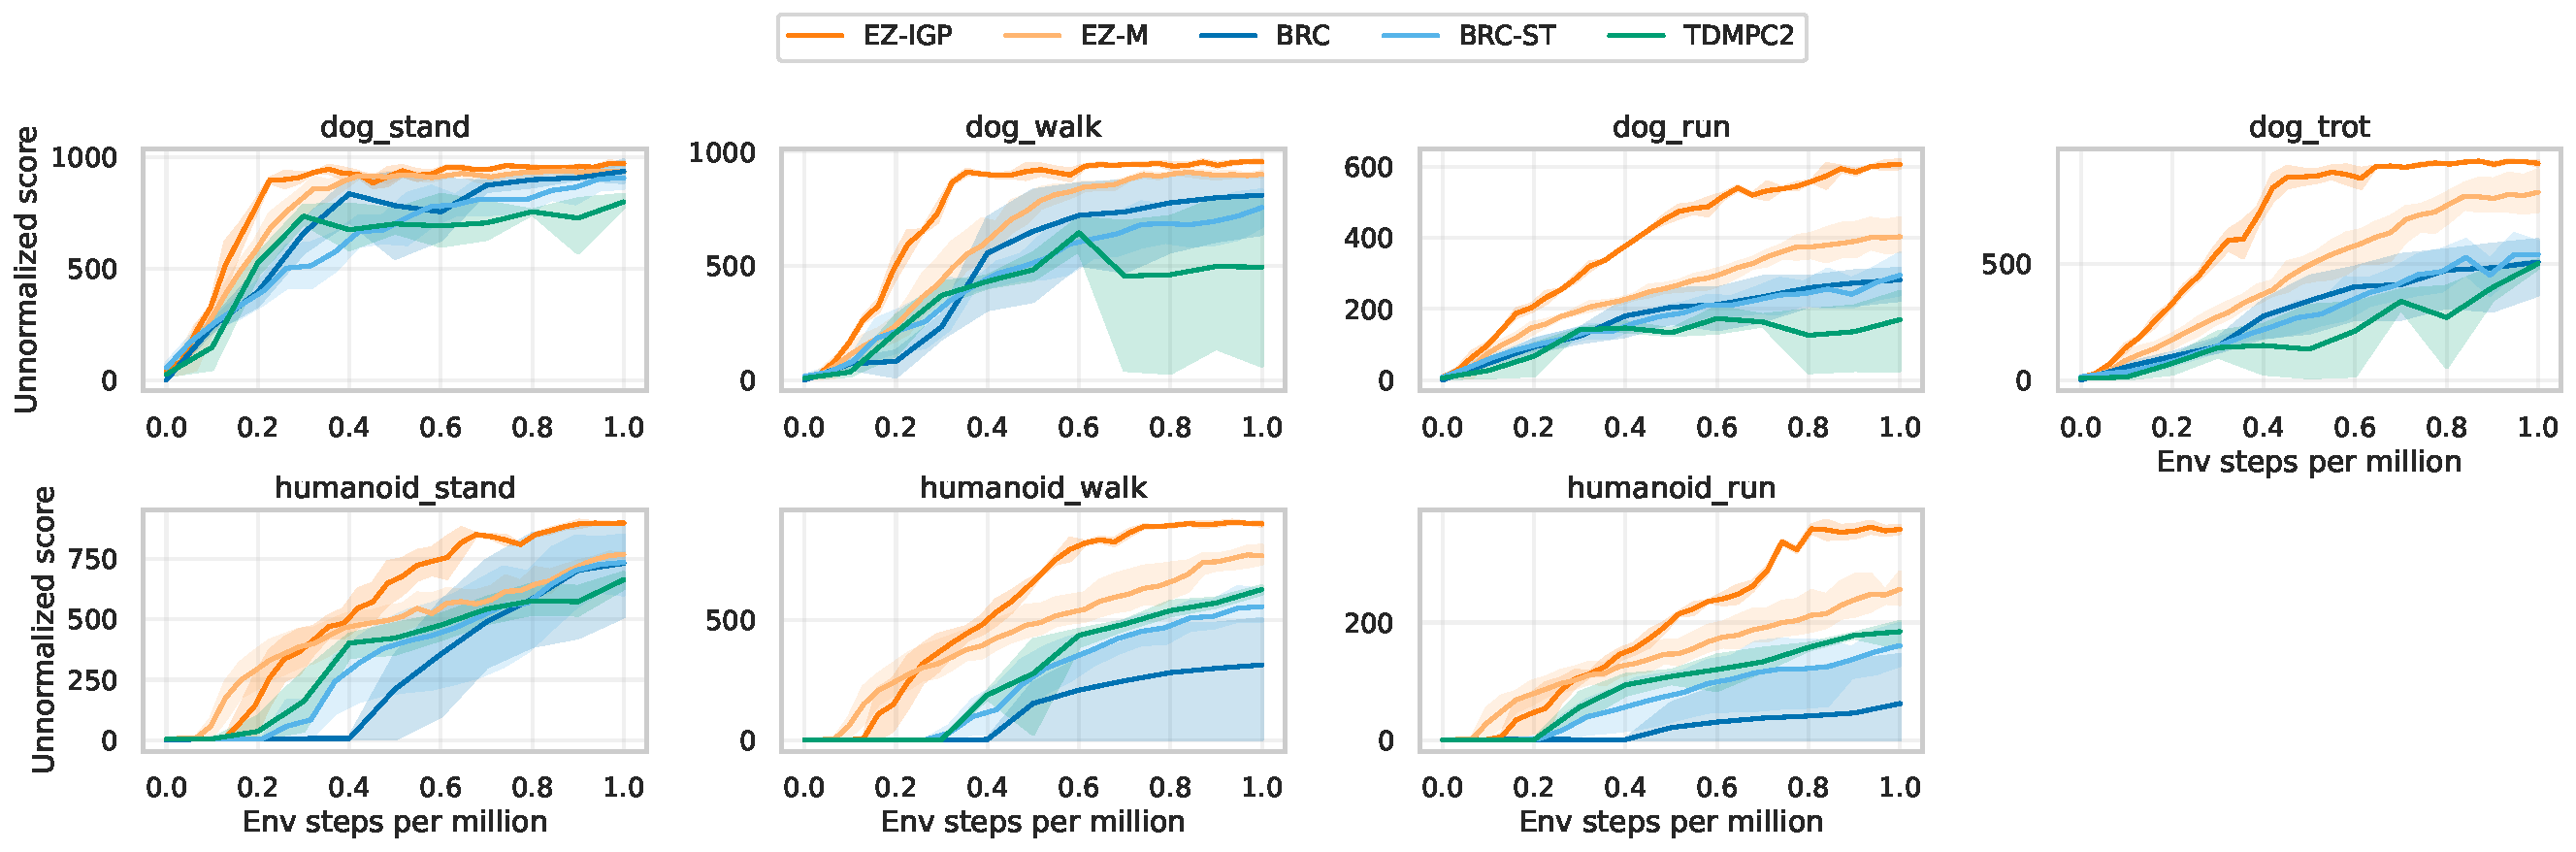
\includegraphics[width=1.0\linewidth]{figs/dmc_unnorm_curves_igp.pdf}
    \caption{\textbf{Unnormalized curves on DMControl Hard tasks.} The \textit{y}-axis denotes episodic return, and the \textit{x}-axis denotes environment steps (millions). Curves are aggregated over five random seeds, and shaded regions denote 95\% confidence intervals. Per-task scores are listed in Table~\ref{tab:dmc_scores_with_igp}.}
    \label{fig:dmc-unnorm-curves}
\end{figure}

Fig.~\ref{fig:hb-unnorm-curves} reports the analogous curves on the 14-task HumanoidBench-Hard suite (H1hand-* with hand control). Compared with DMC-Hard, this setting introduces additional degrees of freedom from finger actuation, more demanding manipulation-style tasks (\textit{sit\_simple}, \textit{sit\_hard}, \textit{balance\_simple}, \textit{balance\_hard}, \textit{reach}), and substantially higher-dimensional observation and action spaces. Beyond confirming the per-task scores in Table~\ref{tab:humanoidbench_hard}, the curves are useful for diagnosing where the gap between EZ-IGP and the strongest baselines opens up during training, and conversely for identifying tasks---such as \textit{h1hand-stair} and \textit{h1hand-sit\_hard}---where the gap is smaller.

\begin{figure}[ht]
    \centering
    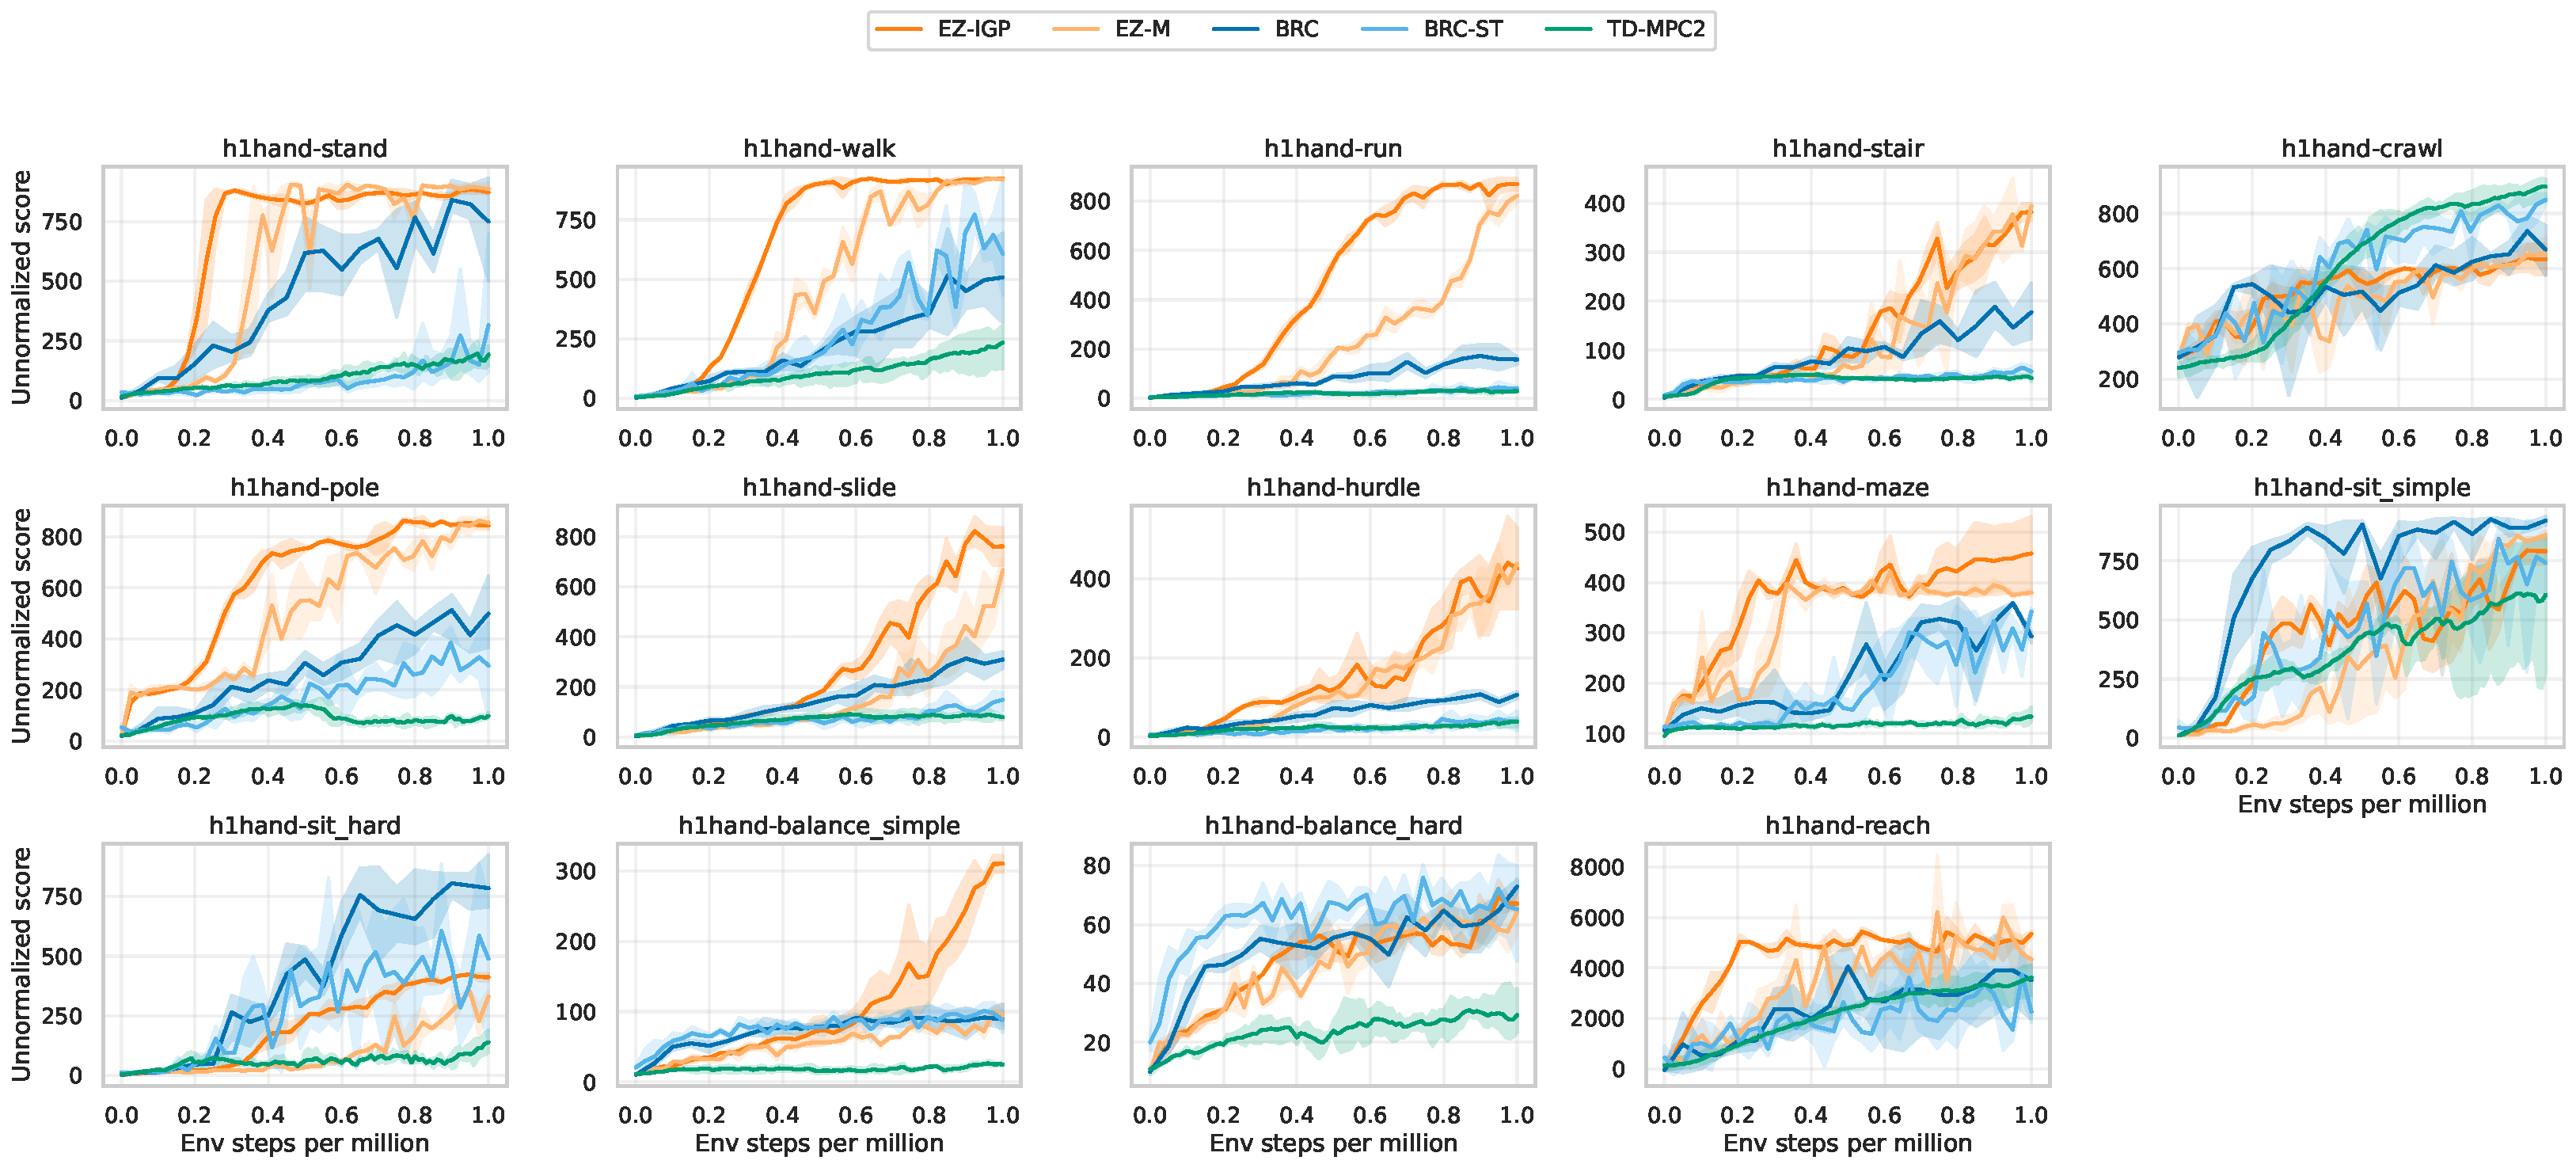
\includegraphics[width=1.0\linewidth]{figs/hard_unnorm_curves_igp.pdf}
    \caption{\textbf{Unnormalized curves on the HumanoidBench-Hard benchmark.} The \textit{y}-axis denotes episodic return, and the \textit{x}-axis denotes environment steps (millions). Curves are aggregated over five random seeds, and shaded regions denote 95\% confidence intervals. Per-task random and success thresholds are listed in Table~\ref{tab:humanoidbench_hard}.}
    \label{fig:hb-unnorm-curves}
\end{figure}


\section{Score Normalization}
\label{app:score-norm}

\paragraph{Why normalize.} The benchmarks we consider span tasks whose raw return scales differ substantially---for example, \texttt{h1hand-reach} has a success score of $1.2\times 10^{4}$ while \texttt{h1hand-walk} has a success score of $700$ (Table~\ref{tab:humanoidbench_hard}). An unweighted average of raw returns across such tasks would be dominated by a handful of large-scale tasks and would obscure relative progress on the rest. Following standard practice in the multi-task RL literature, we therefore normalize each task to a comparable scale before aggregating across tasks.

\paragraph{HumanoidBench normalization.} For each HumanoidBench task we map raw episode return to a normalized score using
\begin{equation}
    \text{Return}_\text{norm}=\frac{\text{Return}-\text{Random Score}}{\text{Success Score}-\text{Random Score}},
\end{equation}
where the \emph{Random Score} is the mean episode return obtained by a uniform-random policy on that task and the \emph{Success Score} is the task-specific completion threshold provided by the benchmark authors. Under this definition, a normalized score of $0$ corresponds to the random baseline and a score of $1$ corresponds to nominal task success; values above $1$ are possible and indicate that the agent exceeds the success threshold. The per-task random and success scores are listed in the first two numerical columns of Table~\ref{tab:humanoidbench_hard}.

\paragraph{DMControl normalization.} DMControl returns are by construction bounded in $[0, 1000]$ on each task, so we adopt the simpler convention of dividing the cumulative reward by $1000$ to obtain a normalized score in $[0, 1]$. This avoids introducing a benchmark-specific random-baseline subtraction that is not part of standard DMControl protocol while keeping DMC and HumanoidBench scores on a comparable scale for cross-benchmark comparisons.

\paragraph{Bolding convention and aggregation.} In Table~\ref{tab:dmc_scores_with_igp} we \textbf{bold} the best result per task. In Table~\ref{tab:humanoidbench_hard} we additionally bold any score that surpasses the per-task success threshold, since multiple methods may simultaneously satisfy this criterion; when no method reaches success, we bold only the SoTA. \textcolor{blue}{For both benchmarks and every method, we take the maximum evaluation return within each seed and task, then report the mean and sample standard deviation across seeds. Benchmark aggregates normalize these per-seed task maxima, average uniformly across tasks within each seed, and finally average across seeds.}


\newpage
\section{Hyperparameters and Details}
\label{app:hyperparameters}

This section documents the implementation details of EZ-IGP needed to reproduce our results. All experiments are conducted on a single machine with 4 NVIDIA A100 GPUs. EZ-IGP is built on top of EZ-M and inherits its multi-task training setup, network architecture, and learning objectives; the only methodological change is replacing the Gaussian policy head with the per-dimension factorized categorical policy and the iterative Gumbel planning procedure. The hyperparameters reported here therefore split naturally into two groups: those inherited from EZ-M (optimization, world-model unrolling, replay) and those specific to IGP (bin count, Gumbel candidate count, refinement rounds).

\paragraph{Computational efficiency.}
EZ-IGP remains computationally comparable to EZ-M. With 2 search rounds, 16 simulations, and 8 samples per round, EZ-IGP takes 0.368s per decision step. In comparison, EZ-M takes 0.375s per decision step with a single search round using 32 simulations and 16 samples. Thus, the additional iterative refinement in EZ-IGP does not introduce noticeable overhead and preserves comparable overall training efficiency.

\paragraph{Configuration philosophy.} Unless otherwise specified, we keep the same hyperparameter configuration across \textit{all} tasks within a benchmark. This is a deliberate choice. A central claim of this paper is that the projection-error issue we identify is structural rather than tuning-dependent, so per-task hyperparameter searches would muddy that claim by allowing implicit task-specific adaptation. The only configuration that varies between settings is the number of training steps, which we scale with the size and difficulty of the task set: $2\times 10^{5}$ for DMC-Hard (7 tasks) and $3\times 10^{5}$ for HumanoidBench-Hard (14 tasks, with finger actuation and a higher-dimensional action space).

\paragraph{World-model and optimization settings.} We use Adam with a learning rate of $1\times 10^{-4}$ and weight decay of $2\times 10^{-5}$, which we found to be stable across all task combinations we tried; we did not perform a per-task learning-rate sweep. The discount factor $\gamma=0.99$ and batch size of $512$ are standard for continuous-control RL at this scale. We use a relatively short unroll of $5$ steps and a matching TD horizon of $5$, matching the choice in EfficientZeroV2 and shorter than what fully model-based methods such as DreamerV3 use; this reflects our reliance on MCTS to extend planning depth at decision time rather than at training time.

\begin{table}[t]
\centering
\caption{Key hyperparameters used in HumanoidBench experiments}
\label{tab:key_hyperparams}
\begin{tabular}{ll}
\toprule
\textbf{Hyperparameter} & \textbf{Value} \\
\midrule
Discount factor $\gamma$ & 0.99 \\
Unroll steps & 5 \\
TD steps & 5 \\
Batch size & 512 \\
Replay buffer size & $1\times 10^{6}$\\
Training steps & $2\times 10^{5}$ (DMC) / $3\times 10^{5}$ (HumanoidBench) \\
\midrule
Network hidden dimension & 512 \\
Task embedding dimension & 128 \\
Task embedding usage & Rep / Dyn / Rew / Policy-Value \\
Number of res blocks & 3 \\
\midrule
MCTS simulations & 16 \\
Top actions & 8 \\
Sampled actions & 8 \\
num bins & 31 \\
num refined rounds & 2 \\
\midrule
Optimizer & Adam \\
Learning rate & $1\times 10^{-4}$ \\
Weight decay & $2\times 10^{-5}$ \\
\bottomrule
\end{tabular}
\end{table}

\paragraph{IGP-specific hyperparameters.} Three hyperparameters are introduced by IGP. The number of bins per dimension, $V=31$, controls the discretization resolution and trades off representation precision against the per-dimension softmax size. A finer grid yields a tighter discretization-error bound but enlarges the categorical support; our ablations show that returns improve from $V=11$ up to $V=31$ and then plateau, motivating $V=31$ as a default. The number of Gumbel Top-$K$ candidates per planning call is $K=8$ (\textit{Sampled actions}); together with $8$ \textit{Top actions} for sequential halving and $16$ MCTS simulations per inner search, this fixes the per-round search budget. \textcolor{blue}{We use two refinement rounds as a practical performance--compute trade-off. One round disables iterative refinement, while four rounds provide only a small, higher-variance gain in the broader HB-Hard sweep and double the search expansions; the preferred setting is therefore not universal.}

\paragraph{Task conditioning and shared backbone.} We retain EZ-M's task-conditioning mechanism unchanged: a $128$-dimensional task embedding is injected into all four learned components of the world model---representation, dynamics, reward, and policy-value. Injection at all four sites keeps the embedding small while ensuring that task-specific physics (in dynamics and reward) and task-specific behavior (in representation and policy-value) can both be expressed. The shared backbone uses a hidden dimension of $512$ and 3 residual blocks, also inherited from EZ-M.
